\documentclass[12pt,letterpaper]{article}
\usepackage{graphicx,textcomp}
\usepackage{natbib}
\usepackage{setspace}
\usepackage{fullpage}
\usepackage{color}
\usepackage[reqno]{amsmath}
\usepackage{amsthm}
\usepackage{fancyvrb}
\usepackage{amssymb,enumerate}
\usepackage[all]{xy}
\usepackage{endnotes}
\usepackage{lscape}
\newtheorem{com}{Comment}
\usepackage{float}
\usepackage{hyperref}
\newtheorem{lem} {Lemma}
\newtheorem{prop}{Proposition}
\newtheorem{thm}{Theorem}
\newtheorem{defn}{Definition}
\newtheorem{cor}{Corollary}
\newtheorem{obs}{Observation}
\usepackage[compact]{titlesec}
\usepackage{dcolumn}
\usepackage{tikz}
\usetikzlibrary{arrows}
\usepackage{multirow}
\usepackage{xcolor}
\newcolumntype{.}{D{.}{.}{-1}}
\newcolumntype{d}[1]{D{.}{.}{#1}}
\definecolor{light-gray}{gray}{0.65}
\usepackage{url}
\usepackage{listings}
\usepackage{color}
\usepackage{graphicx}
\usepackage{wrapfig}
\usepackage{relsize}

\definecolor{codegreen}{rgb}{0,0.6,0}
\definecolor{codegray}{rgb}{0.5,0.5,0.5}
\definecolor{codepurple}{rgb}{0.58,0,0.82}
\definecolor{backcolour}{rgb}{0.95,0.95,0.92}

\lstdefinestyle{mystyle}{
	backgroundcolor=\color{backcolour},   
	commentstyle=\color{codegreen},
	keywordstyle=\color{magenta},
	numberstyle=\tiny\color{codegray},
	stringstyle=\color{codepurple},
	basicstyle=\footnotesize,
	breakatwhitespace=false,         
	breaklines=true,                 
	captionpos=b,                    
	keepspaces=true,                 
	numbers=left,                    
	numbersep=5pt,                  
	showspaces=false,                
	showstringspaces=false,
	showtabs=false,                  
	tabsize=2
}
\lstset{style=mystyle}
\newcommand{\Sref}[1]{Section~\ref{#1}}
\newtheorem{hyp}{Hypothesis}

\title{Problem Set 1}
\date{Due: October 9, 2025}
\author{Rosalie LaCroix}

\begin{document}
	\maketitle
	
	\vspace{1cm}
	\section*{Question 1: Education}

A school counselor was curious about the average of IQ of the students in her school and took a random sample of 25 students' IQ scores. The following is the data set:\\
\vspace{.5cm}

\lstinputlisting[language=R, firstline=42, lastline=42]{PS01MyAnswers.R}  

\vspace{1cm}

\begin{enumerate}
	\item Find a 90\% confidence interval for the average student IQ in the school.\\

\lstinputlisting[language=R, firstline=44, lastline=52]{PS01MyAnswers.R}

\textsmaller[1]{With repeated sampling, 90\% of confidence intervals will contain the population parameters 93.96, 102.92.}
	
	\item Next, the school counselor was curious  whether  the average student IQ in her school is higher than the average IQ score (100) among all the schools in the country.\\ 
	
	\noindent Using the same sample, conduct the appropriate hypothesis test with $\alpha=0.05$.
	
\lstinputlisting[language=R, firstline=66, lastline=78]{PS01MyAnswers.R}

\begin{center}
	\begin{tabular}{ c c c c}
		Diff in Means & Std Error & t & P-Value \\ 
		-1.560 & 2.619 & -0.596 & 0.722 \\     
	\end{tabular}
\end{center}

\textsmaller[1]{The p-value is greater than 0.05, therefore we did not find significant evidence to reject the null hypothesis that the school counselor's school's average student IQ score was higher than the average score among all the schools in the country.}
	
\end{enumerate}

\newpage

	\section*{Question 2: Political Economy}

\noindent Researchers are curious about what affects the amount of money communities spend on addressing homelessness. The following variables constitute our data set about social welfare expenditures in the USA. \\
\vspace{.5cm}


\begin{tabular}{r|l}
	\texttt{State} &\emph{50 states in US} \\
	\texttt{Y} & \emph{per capita expenditure on shelters/housing assistance in state}\\
	\texttt{X1} &\emph{per capita personal income in state} \\
	\texttt{X2} &  \emph{Number of residents per 100,000 that are "financially insecure" in state}\\
	\texttt{X3} &  \emph{Number of people per thousand residing in urban areas in state} \\
	\texttt{Region} &  \emph{1=Northeast, 2= North Central, 3= South, 4=West} \\
\end{tabular}

\vspace{.5cm}
\noindent Explore the \texttt{expenditure} data set and import data into \texttt{R}.
\vspace{.5cm}
\vspace{.5cm}
\begin{itemize}

\item
Please plot the relationships among \emph{Y}, \emph{X1}, \emph{X2}, and \emph{X3}? What are the correlations among them (you just need to describe the graph and the relationships among them)?
\begin{figure}[h]
	\caption{Relationships Among Y, X1, X2, and X3}
	\label{fig:plot_1}
	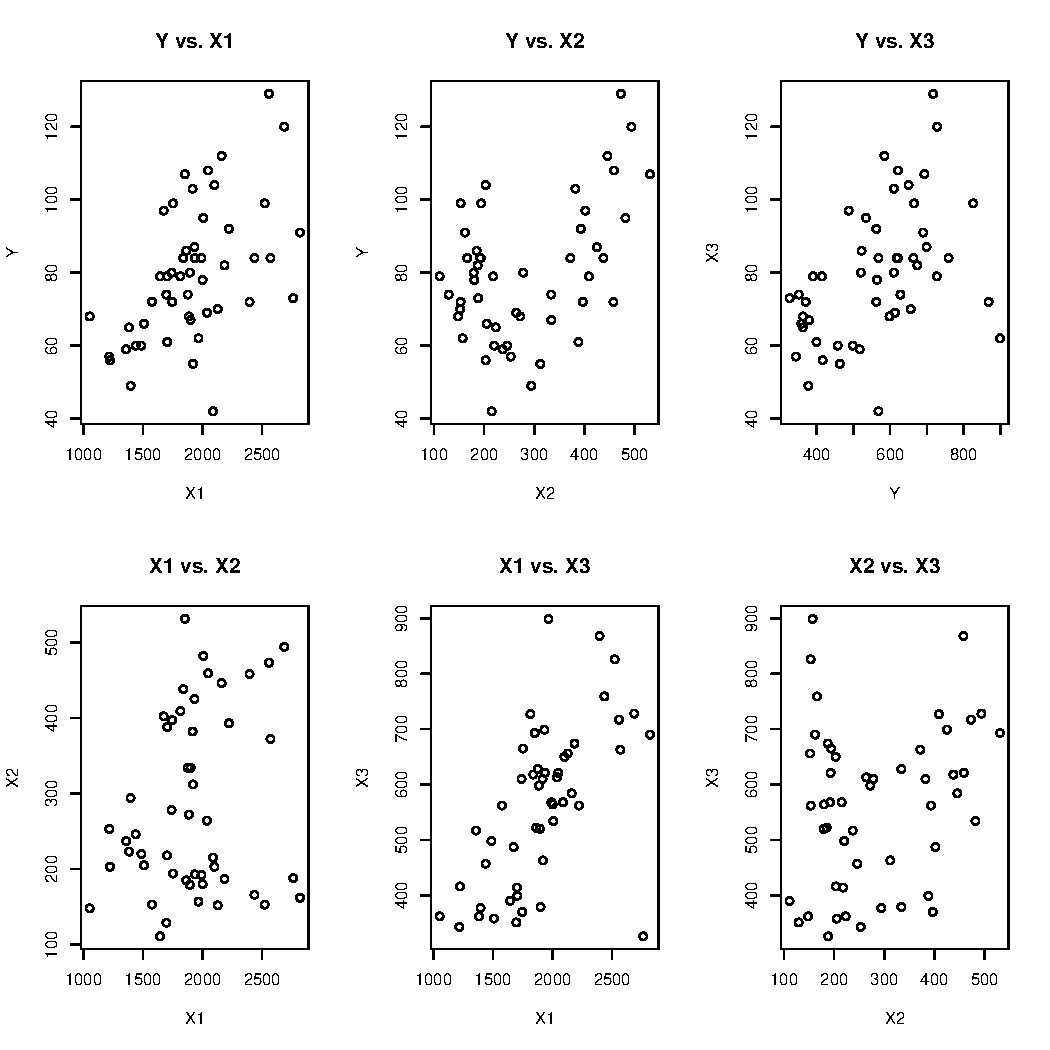
\includegraphics[width=8cm]{six_plots_PS01.pdf}
	\centering
\end{figure}

Y vs. X1
\textsmaller[1]{The graph shows there is a weak to moderate, positive, linear relationship between per capita personal income and per capita expenditure on shelters/housing assistance in states. The reason the relationship is being described as weak to moderate, is that there is a grouping of states that show a stronger positive, linear relationship towards the lower/lower-middle end of the two variables, but as both variables increase, this relationship becomes much weaker.}

Y vs. X2 
\textsmaller[1]{The graph shows that there is little correlation between states' number of residents per 100,000 that are "financially insecure" and the amount of money that state is spending on shelters/housing assistance. Though the general correlation appears minimal, it is important to note that there is a weak, negative, linear correlation between states that have less than 300 residents per 100,000 and their expenditure on shelters/housing assistance. There also appears to be a weak, positive, linear correlation for states that have greater than 400 residents per 100,000 and their expenditure on shelters/housing assistance.}

Y vs. X3
\textsmaller[1]{The graph shows that there is a weak, positive, linear correlation between the per capita expenditure on shelters/housing assistance in a state and it's number of people per thousand residing in urban areas. As Y increases, the relationship appears to weaken further.}

X1 vs. X2
\textsmaller[1]{The graph shows that there is a minimal correlation between states' per capita personal income and the number of residents that are financially there. In states where the per capita personal income is lower, a faint weak, positive correlation can be seen that begins to spread out as per capita personal income increases.}

X1 vs. X3
\textsmaller[1]{The graph shows that there is a weak to moderate, positive, linear relationship between states' per capita personal income and the number of people per thousand residing in rural areas. The correlation weakens when the per capita personal income reaches approximately 2300. There is an outlier from the general trend that appears on the higher end of per capita personal income (X1) but falls very low in the number of people residing in urban areas (X3).}

X2 vs. X3
\textsmaller[1]{The graph shows that there is no correlation between the number of residents that are financially insecure and the number of people residing in urban areas across states.}

\vspace{.5cm}
\item
Please plot the relationship between \emph{Y} and \emph{Region}? On average, which region has the highest per capita expenditure on housing assistance?

\begin{figure}[h]
	\caption{Relationship between Y and Region}
	\label{fig 2:plot_2}
	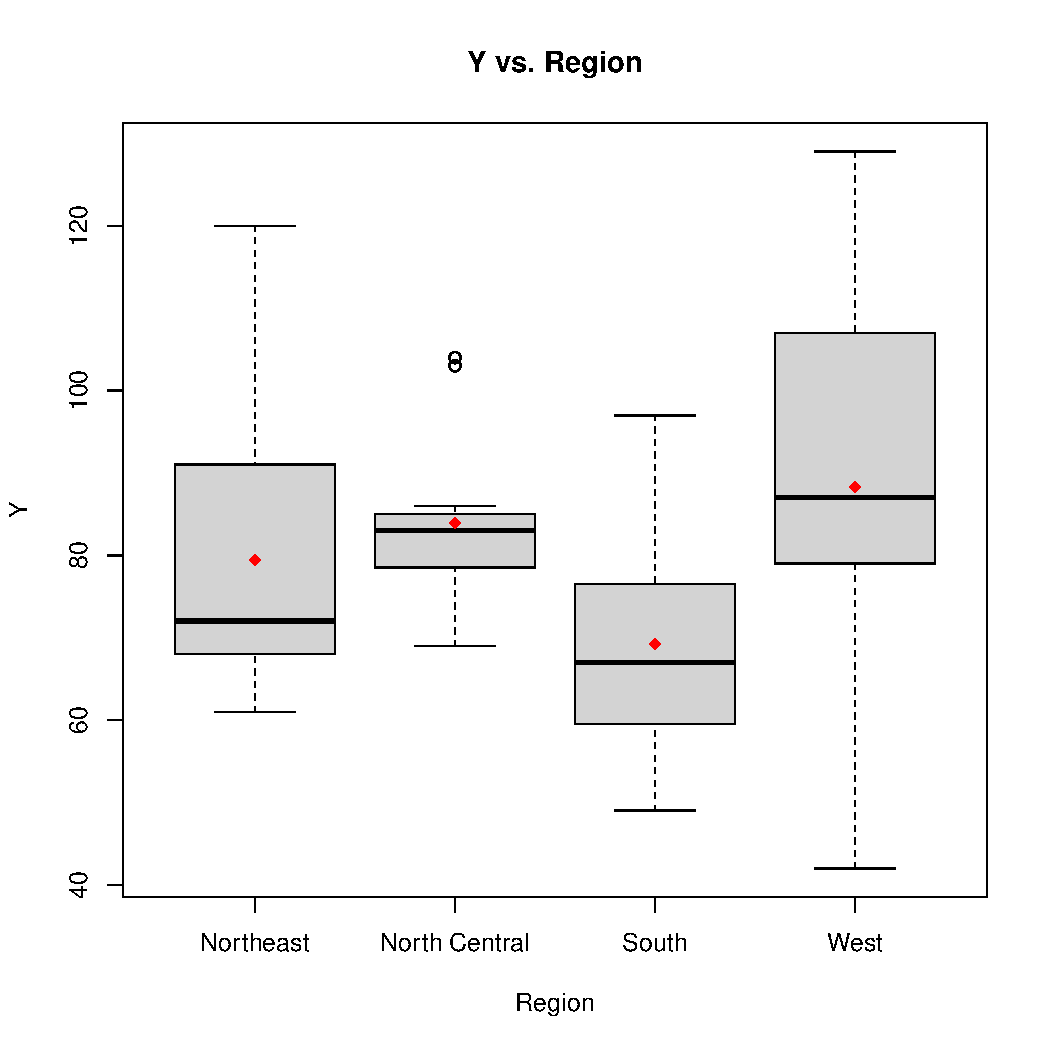
\includegraphics[width=8cm]{y_region_PS01.pdf}
	\centering
\end{figure}

\textsmaller[1]{The West has the highest per capita expenditure on housing assistance. This can be seen in the boxplot with the red dot marking the means of each region.}

\vspace{.5cm}
\item
Please plot the relationship between \emph{Y} and \emph{X1}? Describe this graph and the relationship. Reproduce the above graph including one more variable \emph{Region} and display different regions with different types of symbols and colors.
\begin{figure}[h]
	\caption{Relationship between Personal Income and Spending on Shelters/Housing Assistance in States}
	\label{fig 3:plot_3}
	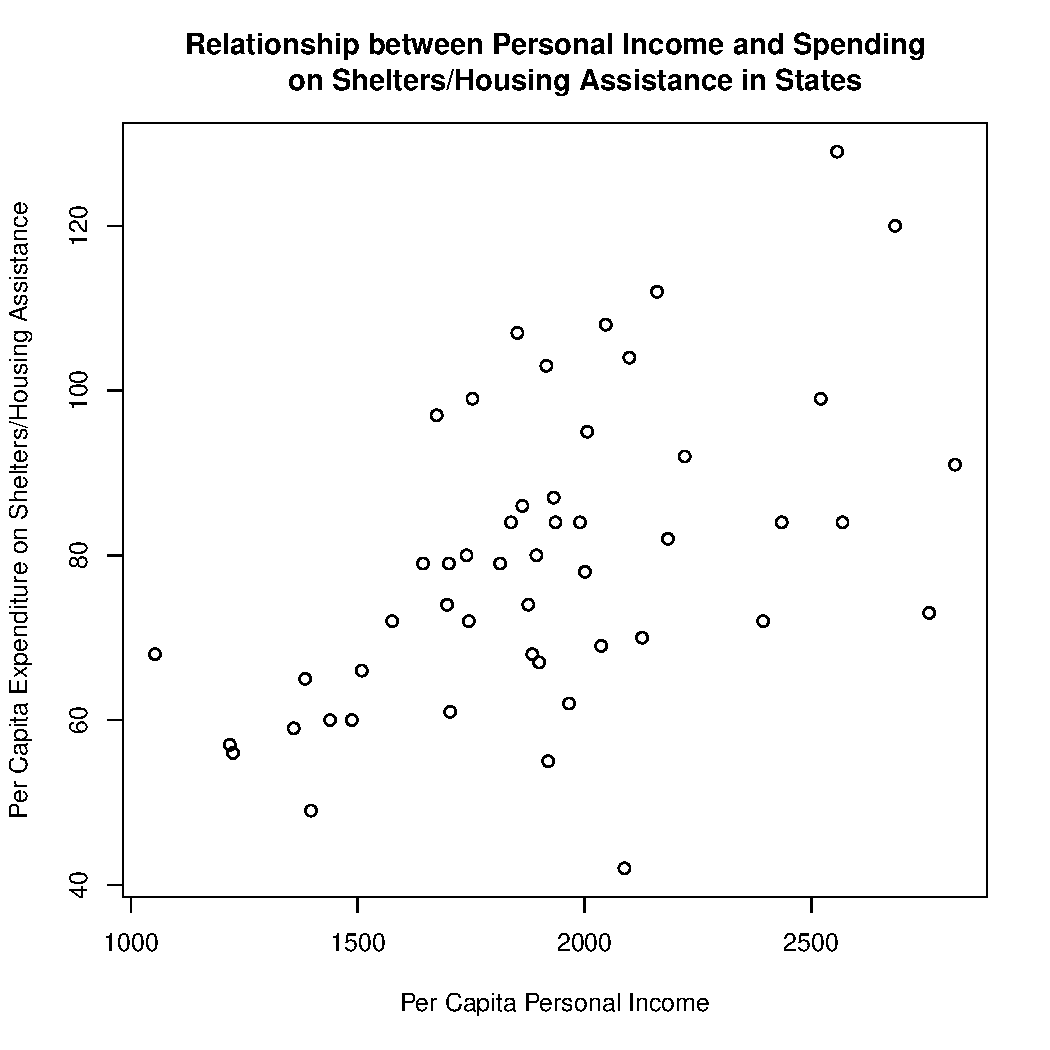
\includegraphics[width=8cm]{original_last_q_PS01.pdf}
	\centering
\end{figure}

\textsmaller[1]{The graph shows there is a weak to moderate, positive, linear relationship between per capita personal income and per capita expenditure on shelters/housing assistance in states. The reason the relationship is being described as weak to moderate, is that there is a grouping of states that show a stronger positive, linear relationship towards the lower/lower-middle end of the two variables, but as both variables increase, this relationship becomes much weaker.}

\begin{figure}[h]
	\caption{Relationship between Personal Income and Spending on Shelters/Housing Assistance in States, including Region Specification}
	\label{fig 4:plot_4}
	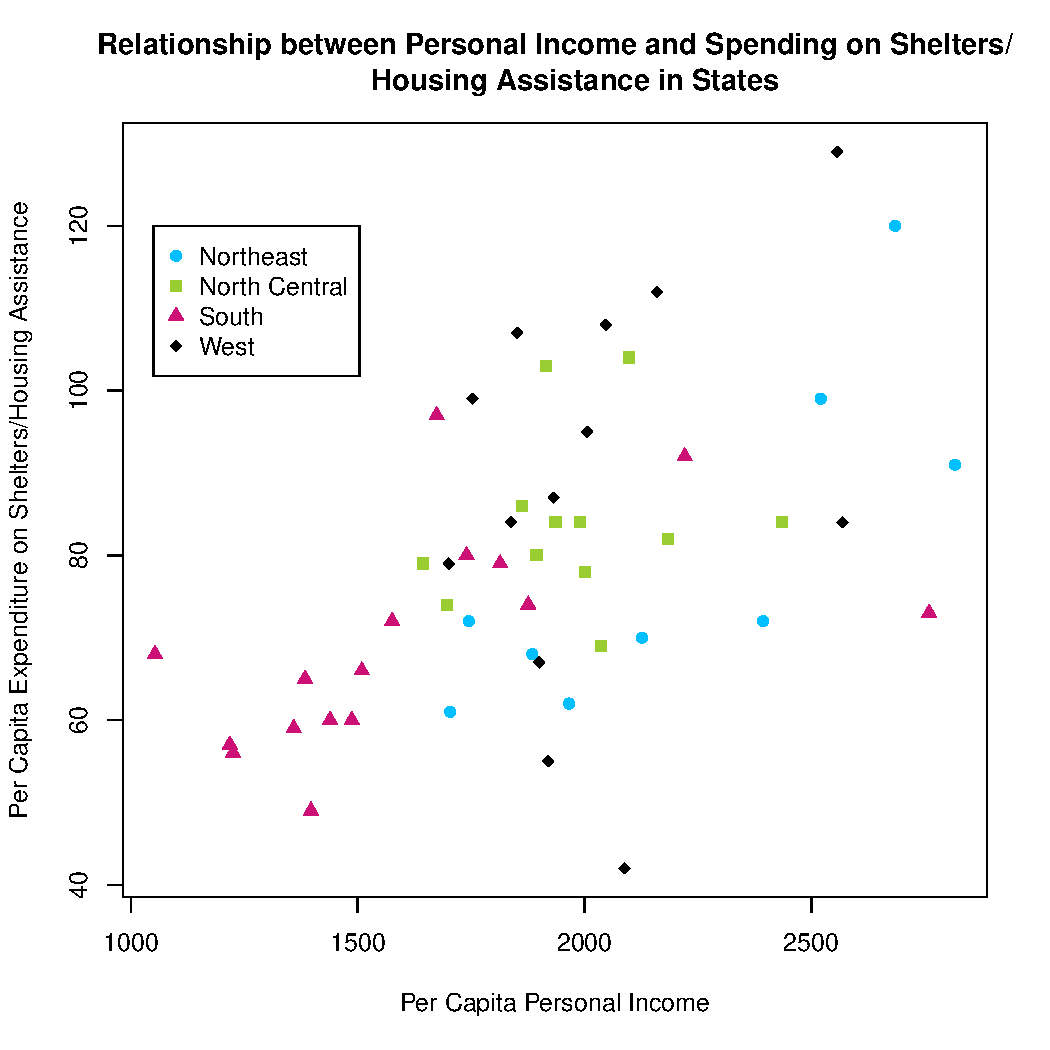
\includegraphics[width=8cm]{last_question_PS01.pdf}
	\centering
\end{figure}
\end{itemize}


\end{document}
